% !TEX encoding = UTF-8 Unicode
% -*- coding: UTF-8; -*-
% vim: set fenc=utf-8
\documentclass[a4paper,12pt,french]{article}

\usepackage{centrale}
\usepackage{algorithm}
\usepackage{algorithmic}
\usepackage{amsmath}

\hypersetup{
    pdftitle={Parareal Algorithm},
    pdfauthor={Oussama BOUHENNICHE},
    pdfsubject={Parareal Algorithm},
    pdfproducer={Conversion PDF à insérer},
    pdfkeywords={Parareal, euler, runge kutta, lorenz system} %
}

\DeclareGraphicsRule{.ai}{pdf}{.ai}{.png} % pour insérer des documents .ai
\graphicspath{ {./img/}} % pour ne pas avoir à ajouter eps/ton-image.jpg

% ------------- Packages spéciaux, nécessaires pour ce rapport, à insérer ici ------------- 


\begin{document}

% --------------------------------------------------------------
%                       Page de garde
% --------------------------------------------------------------

\begin{titlepage}
\begin{center}

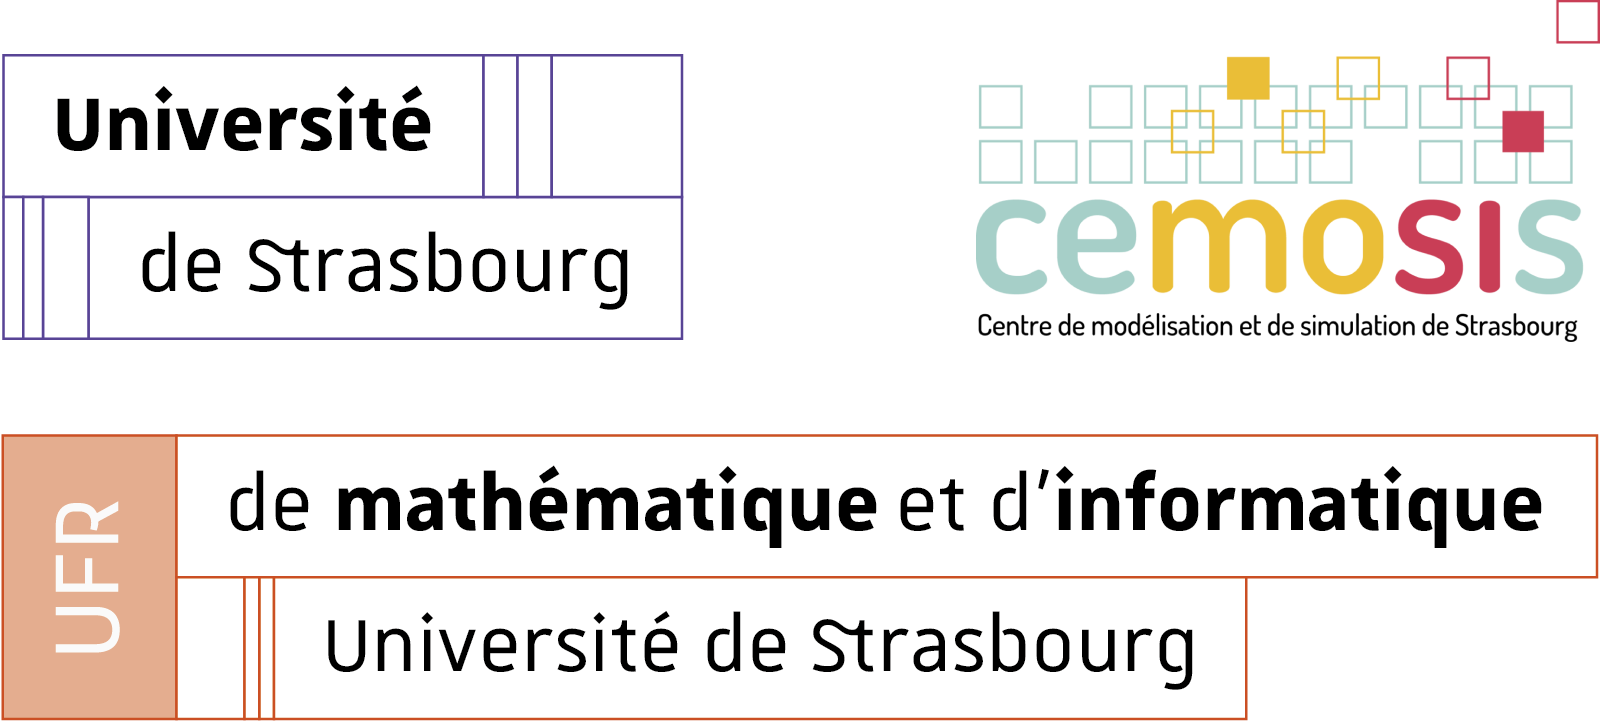
\includegraphics[width=1\textwidth]{logo.png}\\[1cm]

{\large Master 1 CSMI : Scientific Computation and Mathematics of Innovation}\\[0.5cm]

% Title
\rule{\linewidth}{0.5mm} \\[0.4cm]
{ \huge \bfseries Parareal Algorithm: An Advanced Analysis\\[0.4cm] }
\rule{\linewidth}{0.5mm} \\[1.5cm]
% Host Organization
{\large Host Organization: \hyperlink{https://www.cemosis.fr/}{Cemosis}}\\[0.5cm]

% Author and supervisor
\noindent
\begin{minipage}{0.6\textwidth}
  \begin{flushleft} \large
    \emph{Author:}\\
    Oussama \textsc{BOUHENNICHE}
  \end{flushleft}
\end{minipage}%
\begin{minipage}{0.4\textwidth}
  \begin{flushright} \large
    \emph{Supervisor:} \\
    M.~Christophe \textsc{Prud'homme}
  \end{flushright}
\end{minipage}



\vfill

% Bottom of the page
{\today}

\end{center}
\end{titlepage}

% --------------------------------------------------------------
%                            Abstract
% --------------------------------------------------------------
\newpage
\thispagestyle{empty}

\vspace*{\fill}
\noindent\rule[2pt]{\textwidth}{0.5pt}\\
{\textbf{Abstract :}}
The parareal algorithm is a method to solve time-dependent problems in parallel. This report presents an analysis of the Parareal algorithm, focusing on its convergence properties, order of convergence, and performance evaluation in a parallel computing context. Various solver combinations and test cases, including the Lorenz system, are analyzed. Solvers tested include explicit Euler, implicit Euler, explicit RK2, implicit RK2, explicit RK4, and implicit RK4. Results indicate that solver choice significantly affects the parallel efficiency, number of iterations, and convergence behavior of the Parareal algorithm. These findings provide valuable insights into optimizing solver selection for parallel-in-time computations.

\\

{\noindent\textbf{keywords :}}
Parareal, Euler, Runge-Kutta, Lorenz system, convergence order, speedup
\\
\noindent\rule[2pt]{\textwidth}{0.5pt}

\vspace*{\fill}
\newpage

% --------------------------------------------------------------
%                    Table des matières 
% --------------------------------------------------------------

\thispagestyle{empty}
\tableofcontents
\newpage
% list of figures
\listoffigures
% --------------------------------------------------------------
%                         Début du corps
% --------------------------------------------------------------
\newpage
\section{Introduction}
The Parareal algorithm is a parallel-in-time integration method designed to solve time-dependent differential equations efficiently by exploiting parallel computation. This report builds upon a previous project where the Parareal algorithm was studied and implemented, along with various ODE solvers. This internship continues and expands upon that work, aiming to further explore the capabilities and performance of the Parareal algorithm.
\newline
\newline
The primary objectives of this report include:
\begin{enumerate}
    \item Analyzing the convergence of the Parareal algorithm by evaluating the number of iterations required for different solver combinations.
    \item Investigating the order of convergence of the Parareal algorithm based on solver choices.
    \item Evaluating the performance of the Parareal algorithm in relation to the number of processes used.
\end{enumerate}\\

Solvers tested include explicit Euler, implicit Euler, explicit RK2, implicit RK2, explicit RK4, and implicit RK4. These solvers represent a range of explicit and implicit methods with varying computational complexities and stability properties. The performance metrics considered in this study provide a comprehensive evaluation of the Parareal algorithm’s efficiency and effectiveness with different solver combinations.



% --------------------------------------------------------------
%                         Partie 1
% --------------------------------------------------------------

\newpage
\section{Background}
\subsection{Parareal Algorithm}
The parareal algorithm, presented by Lions, Maday, and Turinici in 2001 \cite{lions2001resolution}, is an iterative method designed to parallelize the solution of time-dependent differential equations. It aims to solve problems of the form:
$$
\frac{du}{dt} = f(t,u) \;\;\;,\; u(t_0) = u_0
$$

The key idea is to decompose the time domain into smaller sub-intervals, solve these intervals in parallel using a coarse solver for an initial approximation, and iteratively refine the solution using a fine solver. The algorithm leverages parallel computation to achieve significant speedup, making it particularly useful for long-time integration problems.

\subsubsection*{Parareal Algorithm Steps}

\begin{enumerate}
    \item \textbf{Initialization:}
    \begin{itemize}
        \item Divide the time interval $[t_0,T]$ into $N$ sub-intervals: $$t_0<t_1<...<t_N=T$$.
        \item Set the initial guess for the solution at each time point using a coarse solver $G$:
            $$u^0_0=u_0,U^0_n=G(u_{n-1},\Delta t) \text{   for  } n=1,2,...,N$$
    \end{itemize}
    \item \textbf{Iterative Refinement:}
    \begin{itemize}
        \item For each iteration $k$:
        $$u^{k+1}_0=u_0$$
        $$ U_{n+1}^k = G(t_n,t_{n+1},U_n^k) + F(t_n,t_{n+1},U_n^{k-1}) -G(t_n,t_{n+1},U_n^{k-1})\text{   for  } n=1,2,...,N$$
        Here, $G$ is the coarse solver and $F$ is the fine solver. The fine solver $F$ provides a more accurate solution over the sub-interval $\Delta t$.
    \end{itemize}
    \item \textbf{Convergence:}
    \begin{itemize}
        \item The iterations continue until the difference between successive iterations meets a specified tolerance:
        $$||U_n^{k+1}-U_n^{k}|| < tol \text{  for all  } n$$
    \end{itemize}
\end{enumerate}

\subsection{ODEs}

\subsubsection{Lorenz System}
The Lorenz system \cite{lorenz1963deterministic} is used to measure execution time and speedup. It is governed by the following equations:

\begin{equation}
\large
\begin{cases}
    \displaystyle\frac{dx}{dt} = \sigma(y - x) \\
    \displaystyle\frac{dy}{dt} = x(\rho - z) - y \\
    \displaystyle\frac{dz}{dt} = xy - \beta z
\end{cases}
\normalsize
\end{equation}\\
   
where:
\begin{itemize}
    \item $x$ is the rate of convective overturning,
    \item $y$ is the horizontal temperature variation,
    \item $z$ is the vertical temperature variation,
    \item $\sigma$ is the Prandtl number,
    \item $\rho$ is the Rayleigh number,
    \item $\beta$ is a geometrical factor.
\end{itemize}

The equations describe the behavior of a two-dimensional fluid layer that is heated uniformly from below and cooled from above.\\
   
\begin{itemize}
    \item Parameters: $\sigma=10$, $\rho=28$, $\beta=\frac{8}{3}$.
    \item Initial conditions: $u_0=[5,-5,20]$.
    \item Time span: $[0,10]$.
\end{itemize}

We used the parameters and initial condition proposed by H Batmalle, PE Bécue, V Le Gallic (2011),\cite{batmalle2011acceleration}

\subsubsection{Other Test Systems}
These systems are used to measure the number of Parareal iterations required for convergence and the convergence order.

\begin{itemize}
    \item \textbf{System 1:} \newline \begin{equation}
            \frac{dy}{dt} = -ty^2
            \end{equation}
            \begin{itemize}
                \item Exact solution: $y(t)=\frac{2}{1+t^2}$.
                \item Initial condition: $y(0)=2$.
                \item Time span: $[0,5]$.
            \end{itemize}
    \item \textbf{System 2:} \newline \begin{equation}
            \frac{dy}{dt} = -y+ cos(t)
            \end{equation}
            \begin{itemize}
                \item Exact solution: $y(t)=\frac{-1}{2}e^{-t}+\frac{1}{2}cos(t)+\frac{1}{2}sin(t)$.
                \item Initial condition: $y(0)=0$.
                \item Time span: $[0,5]$.
            \end{itemize}
    \item \textbf{System 1:} \newline \begin{equation}
            \frac{dy}{dt} = -2y
            \end{equation}
            \begin{itemize}
                \item Exact solution: $y(t)=e^{-2t}$.
                \item Initial condition: $y(0)=1$.
                \item Time span: $[0,5]$.
            \end{itemize}
\end{itemize}

%\begin{listing}[ht]
%\inputminted[mathescape,
               %numbersep=5pt,
               %gobble=2,
               %frame=lines,
               %framesep=2mm]{python}{code/}
%\caption{Du code informatique}
%\label{listing:id-du-code}
%\end{listing}

\subsection{Solvers}
Six different solvers were tested, representing a mix of explicit and implicit methods with varying computational complexities and stability properties \cite{suli2010numerical}.
\subsubsection{Explicit Euler (feuler)}
\begin{itemize}
    \item \textbf{Order:} First-order.
    \item \textbf{Stability:} Conditionally stable.
    \item \textbf{Scheme:} \begin{equation}
        y_{n+1}=y_n+h*f(t_n,y_n)
    \end{equation}
\end{itemize}

\subsubsection{Implicit Euler (beuler)}
This requires solving a nonlinear equation at each step, typically using fixed-point iteration or Newton's method.
\begin{itemize}
    \item \textbf{Order:} First-order.
    \item \textbf{Stability:} Unconditionally stable.
    \item \textbf{Scheme:} \begin{equation}
        y_{n+1}=y_n+h*f(t_{n+1},y_{n+1})
    \end{equation}
\end{itemize}

\subsubsection{Explicit RK2 (rk2)}
\begin{itemize}
    \item \textbf{Order:} Second-order.
    \item \textbf{Stability:} Conditionally stable..
    \item \textbf{Scheme:} 
        \begin{equation*}
            k_1=hf(t_n,y_n)
        \end{equation*}
        \begin{equation*}
            k_2=hf(t_n+h,y_n+k_1)
        \end{equation*}
        \begin{equation}
            y_{n+1}=y_n+\frac{1}{2}(k_1+k_2)
        \end{equation}

\end{itemize}

\subsubsection{Implicit RK2 (brk2)}
This also involves solving a nonlinear system at each step.
\begin{itemize}
    \item \textbf{Order:} Second-order.
    \item \textbf{Stability:} Unconditionally stable.
    \item \textbf{Scheme:} \begin{equation}
        y_{n+1}=y_n+hf(t_n+2h,y_n+2hf(t_n,yn))
    \end{equation}
\end{itemize}

\subsubsection{Explicit RK4 (rk4)}
\begin{itemize}
    \item \textbf{Order:} Fourth-order.
    \item \textbf{Stability:} Conditionally stable..
    \item \textbf{Scheme:}
        \begin{equation*}
            k_1=hf(t_n,y_n)
        \end{equation*}
        \begin{equation*}
            k_2=hf(t_n+\frac{h}{2},y_n+\frac{k_1}{2})
        \end{equation*}
        \begin{equation*}
            k_3=hf(t_n+\frac{h}{2},y_n+\frac{k_2}{2})
        \end{equation*}
        \begin{equation*}
            k_4=hf(t_n+h,y_n+k_3)
        \end{equation*}
        \begin{equation}
            y_{n+1}=y_n+\frac{1}{6}(k_1+2k_2+2k_3+k_4)
        \end{equation}

\end{itemize}

\subsubsection{Implicit RK4 (brk4)}
This involves solving a complex system of nonlinear equations.
\begin{itemize}
    \item \textbf{Order:} Fourth-order.
    \item \textbf{Stability:} Unconditionally stable.
    \item \textbf{Scheme:} \begin{multline}
        y{n+1}=y_n+\frac{h}{6}(f(t_n,y_n)+2f(t_n+\frac{h}{2},y_n+\frac{h}{2}f(t_n,y_n)) \\ +2f(t_n+\frac{h}{2},y_n+\frac{h}{2}f(t_n+\frac{h}{2},y_n+\frac{h}{2}f(t_n,y_n))) \\ +f(t_n+h,y_n+hf(t_n+\frac{h}{2},y_n+\frac{h}{2}f(t_n,y_n))))
    \end{multline}
\end{itemize}

% --------------------------------------------------------------
%                            Partie 2
% --------------------------------------------------------------


\
\section{Methodology}
\subsection{Host Organization}
\subsubsection{Overview}
The internship was hosted by \hyperlink{https://www.cemosis.fr/}{Cemosis}, a research laboratory specializing in scientific computing, mathematical modeling, and industrial applications. Cemosis collaborates closely with academic institutions and industry partners to develop innovative solutions in computational science and engineering.
\subsubsection{Access to Resources}
Access to high-performance computing resources and specialized software tools facilitated the implementation and testing of the Parareal algorithm across different solver configurations and test cases. This infrastructure enabled rigorous experimentation and performance evaluation under varying computational loads.
\subsection{Experimental Setup}
\subsubsection{Parallel Environment}
The experiments were conducted on a computing cluster utilizing many threads to parallelize the Parareal algorithm across multiple cores.

\subsubsection{Solver Configurations}
Each test case employed a combination of coarse and fine solvers. These solvers were selected based on their computational complexity, stability characteristics, and order of convergence to provide a comprehensive evaluation of the Parareal algorithm's performance.

\subsubsection{Convergence Criteria}
The convergence of the Parareal algorithm was assessed based on the $\boldsymbol\ell^2$ norm of the difference between successive iterations of the solution vector. Convergence was deemed achieved when the difference fell below a predefined tolerance level \textit{tol}.

\subsection{Tests Setup}
\subsubsection{Number of Parareal Iterations and Convergence Order Tests}
To assess the number of iterations required for convergence and to determine the convergence order, the different systems (System 1, System 2, System 3) were tested.
The steps for these tests were:
\begin{enumerate}
    \item \textbf{Initial Setup:}
        \begin{itemize}
            \item For each system, the initial condition was set as specified.
            \item The time span $[0,5]$ was discretized into appropriate time intervals.
        \end{itemize}
    \item \textbf{Execution:}
        \begin{itemize}
            \item For each system, numerical solutions were obtained using different solver combinations (Explicit Euler, Implicit Euler, Explicit RK2, Implicit RK2, Explicit RK4, Implicit RK4).
            \item The number of Parareal iterations required to reach a specified tolerance \textit{tol}. was recorded for each solver combination.
        \end{itemize}
    \item \textbf{Convergence Order:}
        \begin{itemize}
            \item The convergence order was determined by comparing the numerical solutions to the exact solutions obtained analytically.
            \item The difference between the numerical and exact solutions was analyzed to assess the convergence behavior.
        \end{itemize}
\end{enumerate}

\subsubsection{Execution Time and Speedup Tests}
To evaluate the execution time and speedup, the Lorenz system was used.
The steps for these tests were:
\begin{enumerate}
    \item \textbf{Initial Setup:}
        \begin{itemize}
            \item The initial condition and parameters were set as specified.
            \item he time span $[0,10]$ was discretized into appropriate time intervals.
        \end{itemize}
    \item \textbf{Parallel Execution:}
        \begin{itemize}
            \item The Lorenz system was solved using different numbers of processes ($P$) with MPI for parallel execution.
            \item Execution times ($T_P$) were recorded for each $P$.
        \end{itemize}
    \item \textbf{Speedup Calculation:}
        \begin{itemize}
            \item Speedup ($S$) was calculated using the formula:
                \begin{equation}
                    S = \frac{T_1}{T_p}
                \end{equation}
        \end{itemize}
        where $T_1$ is the execution time with 1 process, and $T_P$ is the execution time with $P$ processes.
\end{enumerate}

\section{Results and Analysis}
This section presents the results from the tests conducted using the Parareal algorithm with various solver combinations. The focus is on convergence analysis, order of convergence, and performance evaluation in a parallel computing environment.

\subsection{Convergence Analysis}
To evaluate the convergence of the Parareal algorithm, three systems were tested: System 1, System 2, and System 3. Each system was solved using different solver combinations, and the number of iterations required to reach a specified tolerance (\textit{tol}) was recorded.
\subsubsection{Number of Parareal Iterations for Convergence}
The results for the number of iterations required by the Parareal algorithm to converge using different combinations of coarse and fine solvers are presented below for the three different systems. The results are depicted in the provided bar charts.
\newline
\newline
\textbf{System 1 Results:}
\begin{figure}[ht!]
    \centering
    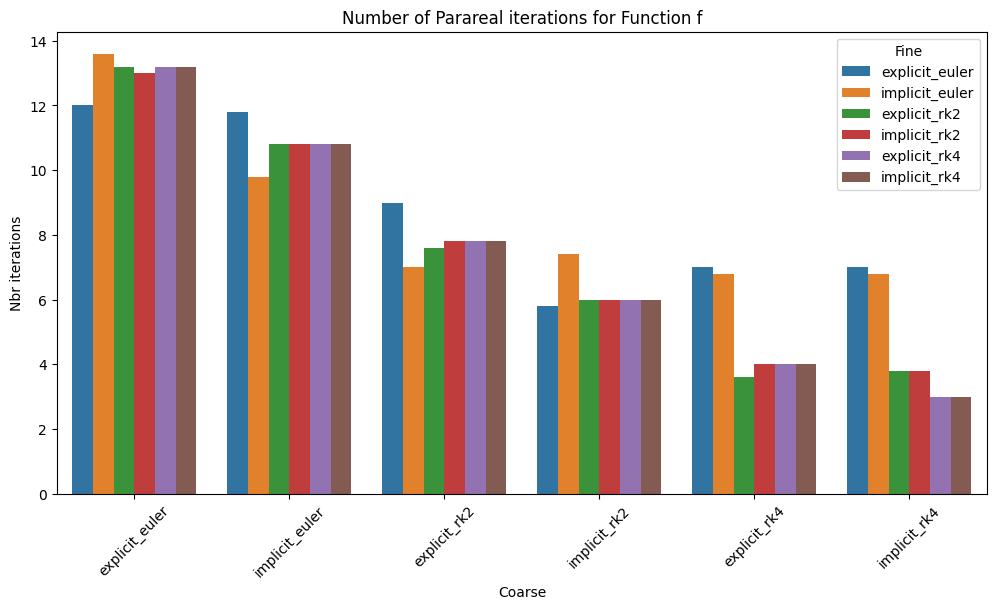
\includegraphics[width=.85\textwidth]{img/nbr_iter_f.png}
    \caption{Number of Parareal iterations for system 1}
    \label{fig:1}
\end{figure}
\newpage
\textbf{System 2 Results:}
\begin{figure}[ht!]
    \centering
    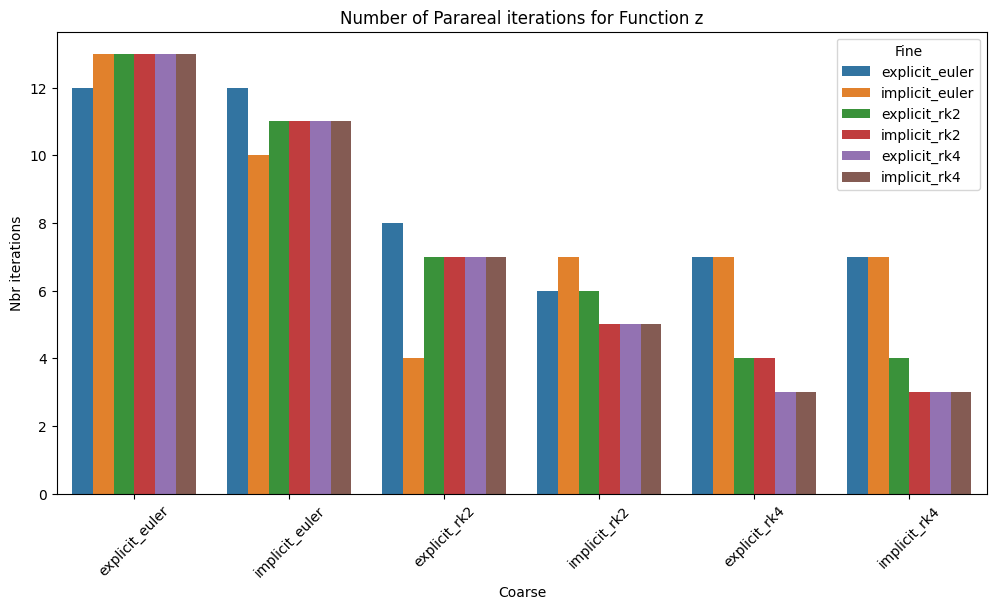
\includegraphics[width=.85\textwidth]{img/nbr_iter_z.png}
    \caption{Number of Parareal iterations for system 2}
    \label{fig:2}
\end{figure}
\newline
\textbf{System 3 Results:}
\begin{figure}[ht!]
    \centering
    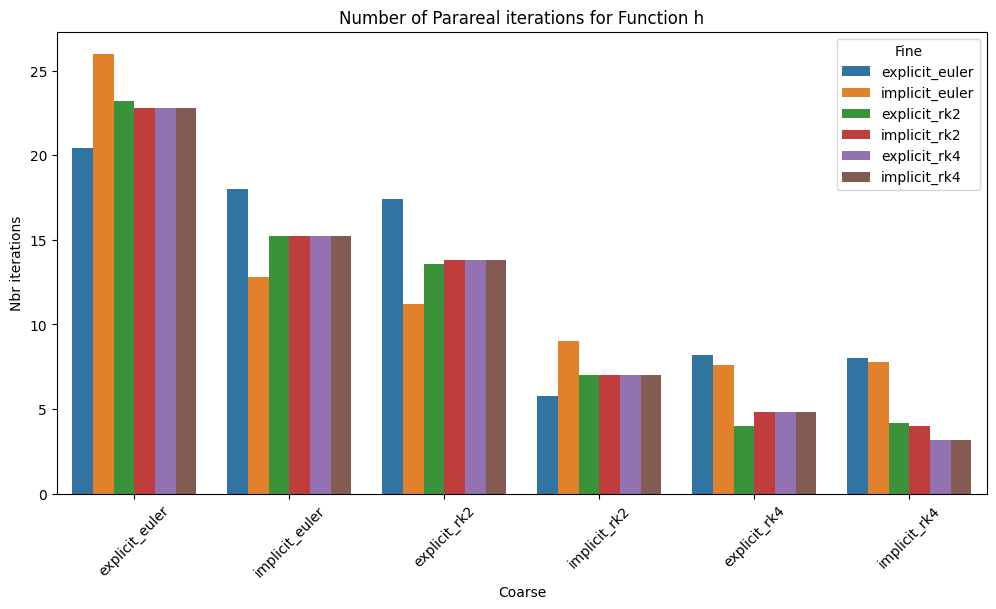
\includegraphics[width=.85\textwidth]{img/nbr_iter_h.png}
    \caption{Number of Parareal iterations for system 3}
    \label{fig:3}
\end{figure}

\newpage
\textbf{Analysis:}
\begin{itemize}
    \item The number of iterations required for convergence varied significantly depending on the solver combination used.
    \item Higher-order coarse solvers tended to require fewer iterations for convergence compared to lower-order solvers.
    \item Explicit Euler required the most iterations across all systems, indicating lower efficiency in the Parareal framework.
    \item Implicit methods generally led to faster convergence, with implicit RK4 requiring the least number of iterations.
    \item The choice of the coarse solver affect the number of iterations required for convergence and Parareal using Higher-order coarse solvers tended to converge faster than lower-order.
\end{itemize}
\subsection{Order of Convergence}
The order of convergence was analyzed by comparing the numerical solutions obtained using the Parareal algorithm to the exact solutions of the test systems.
\subsubsection{Convergence Order Results}
The following figures illustrate the results of convergence order test for the different systems using various solvers combinations. The results are presented in the provided bar charts.
\newline
\newpage
\textbf{System 1 Results:}
\begin{figure}[ht!]
    \centering
    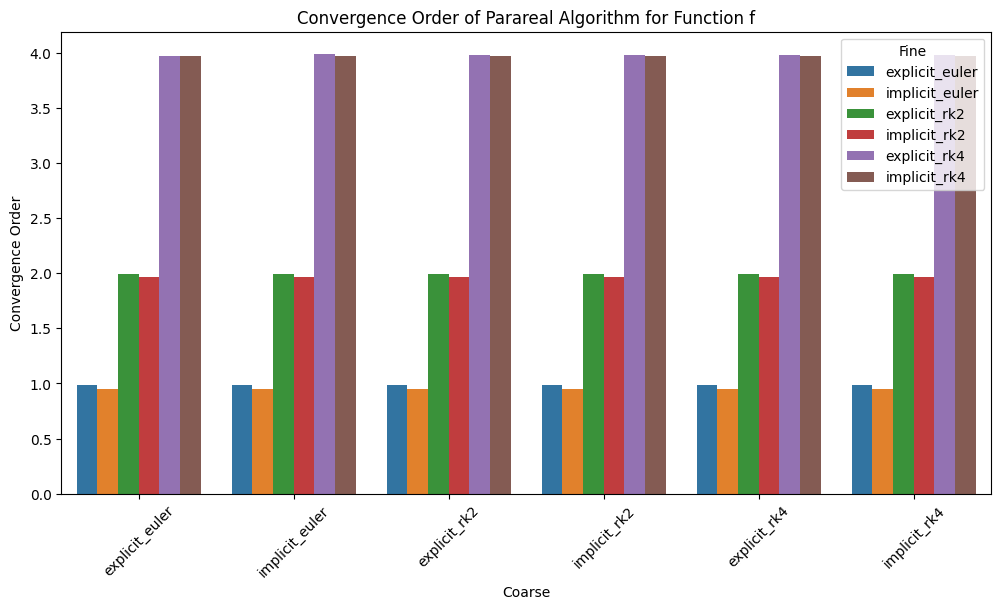
\includegraphics[width=.92\textwidth]{img/cv_ord_f.png}
    \caption{Convergence Order of Parareal Algorithm for system 1}
    \label{fig:4}
\end{figure}

\textbf{System 2 Results:}
\begin{figure}[ht!]
    \centering
    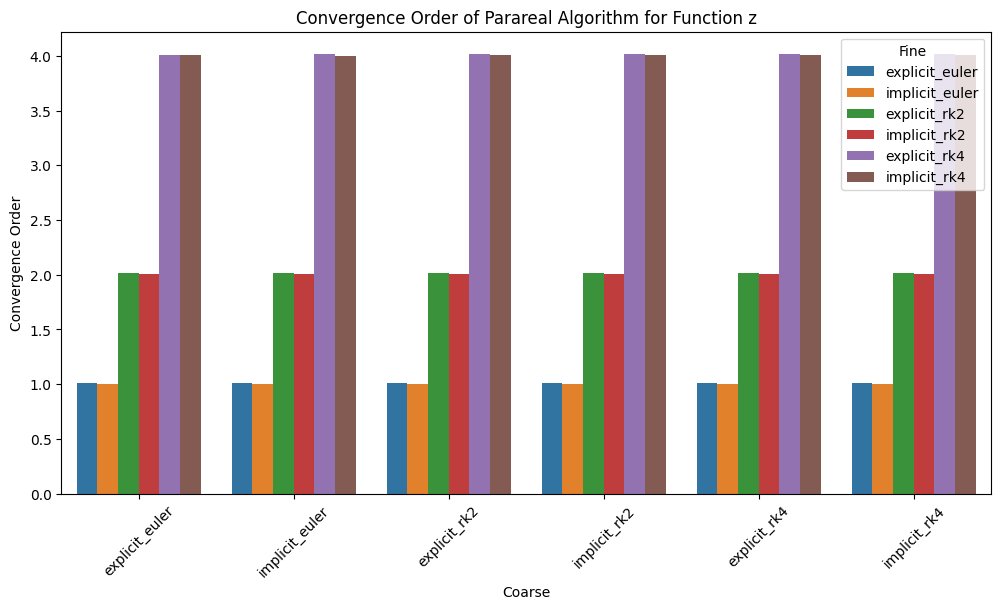
\includegraphics[width=.92\textwidth]{img/cv_ord_z.png}
    \caption{Convergence Order of Parareal Algorithm for system 2}
    \label{fig:5}
\end{figure}
\newline

\textbf{System 3 Results:}
\begin{figure}[ht!]
    \centering
    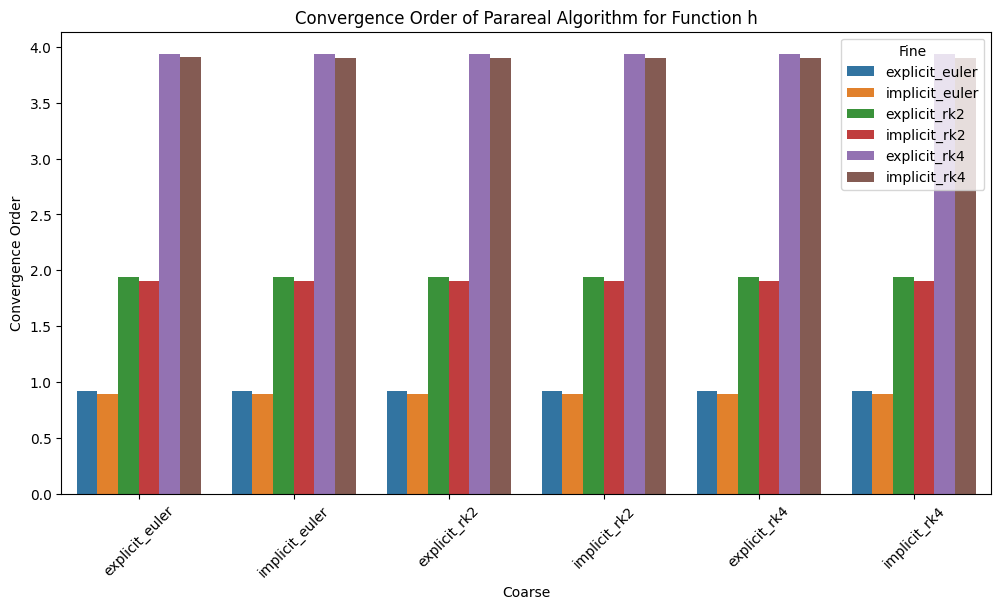
\includegraphics[width=.92\textwidth]{img/cv_ord_h.png}
    \caption{Convergence Order of Parareal Algorithm for system 3}
    \label{fig:6}
\end{figure}

\textbf{Analysis:}
\begin{itemize}
    \item The order of convergence of the Parareal algorithm is primarily set by the fine solver used in the iterative process. This means that the accuracy and efficiency of the Parareal algorithm are directly influenced by the characteristics of the fine solver.
    \item  Higher-order fine solvers lead to a higher order of convergence for the overall algorithm.
\end{itemize}

\subsection{Performance Evaluation}
The performance of the Parareal algorithm was evaluated using the Lorenz system to measure execution time and speedup achieved with parallel execution.
\subsubsection{Execution Time and Speedup}

\begin{figure}[ht!]
    \centering
    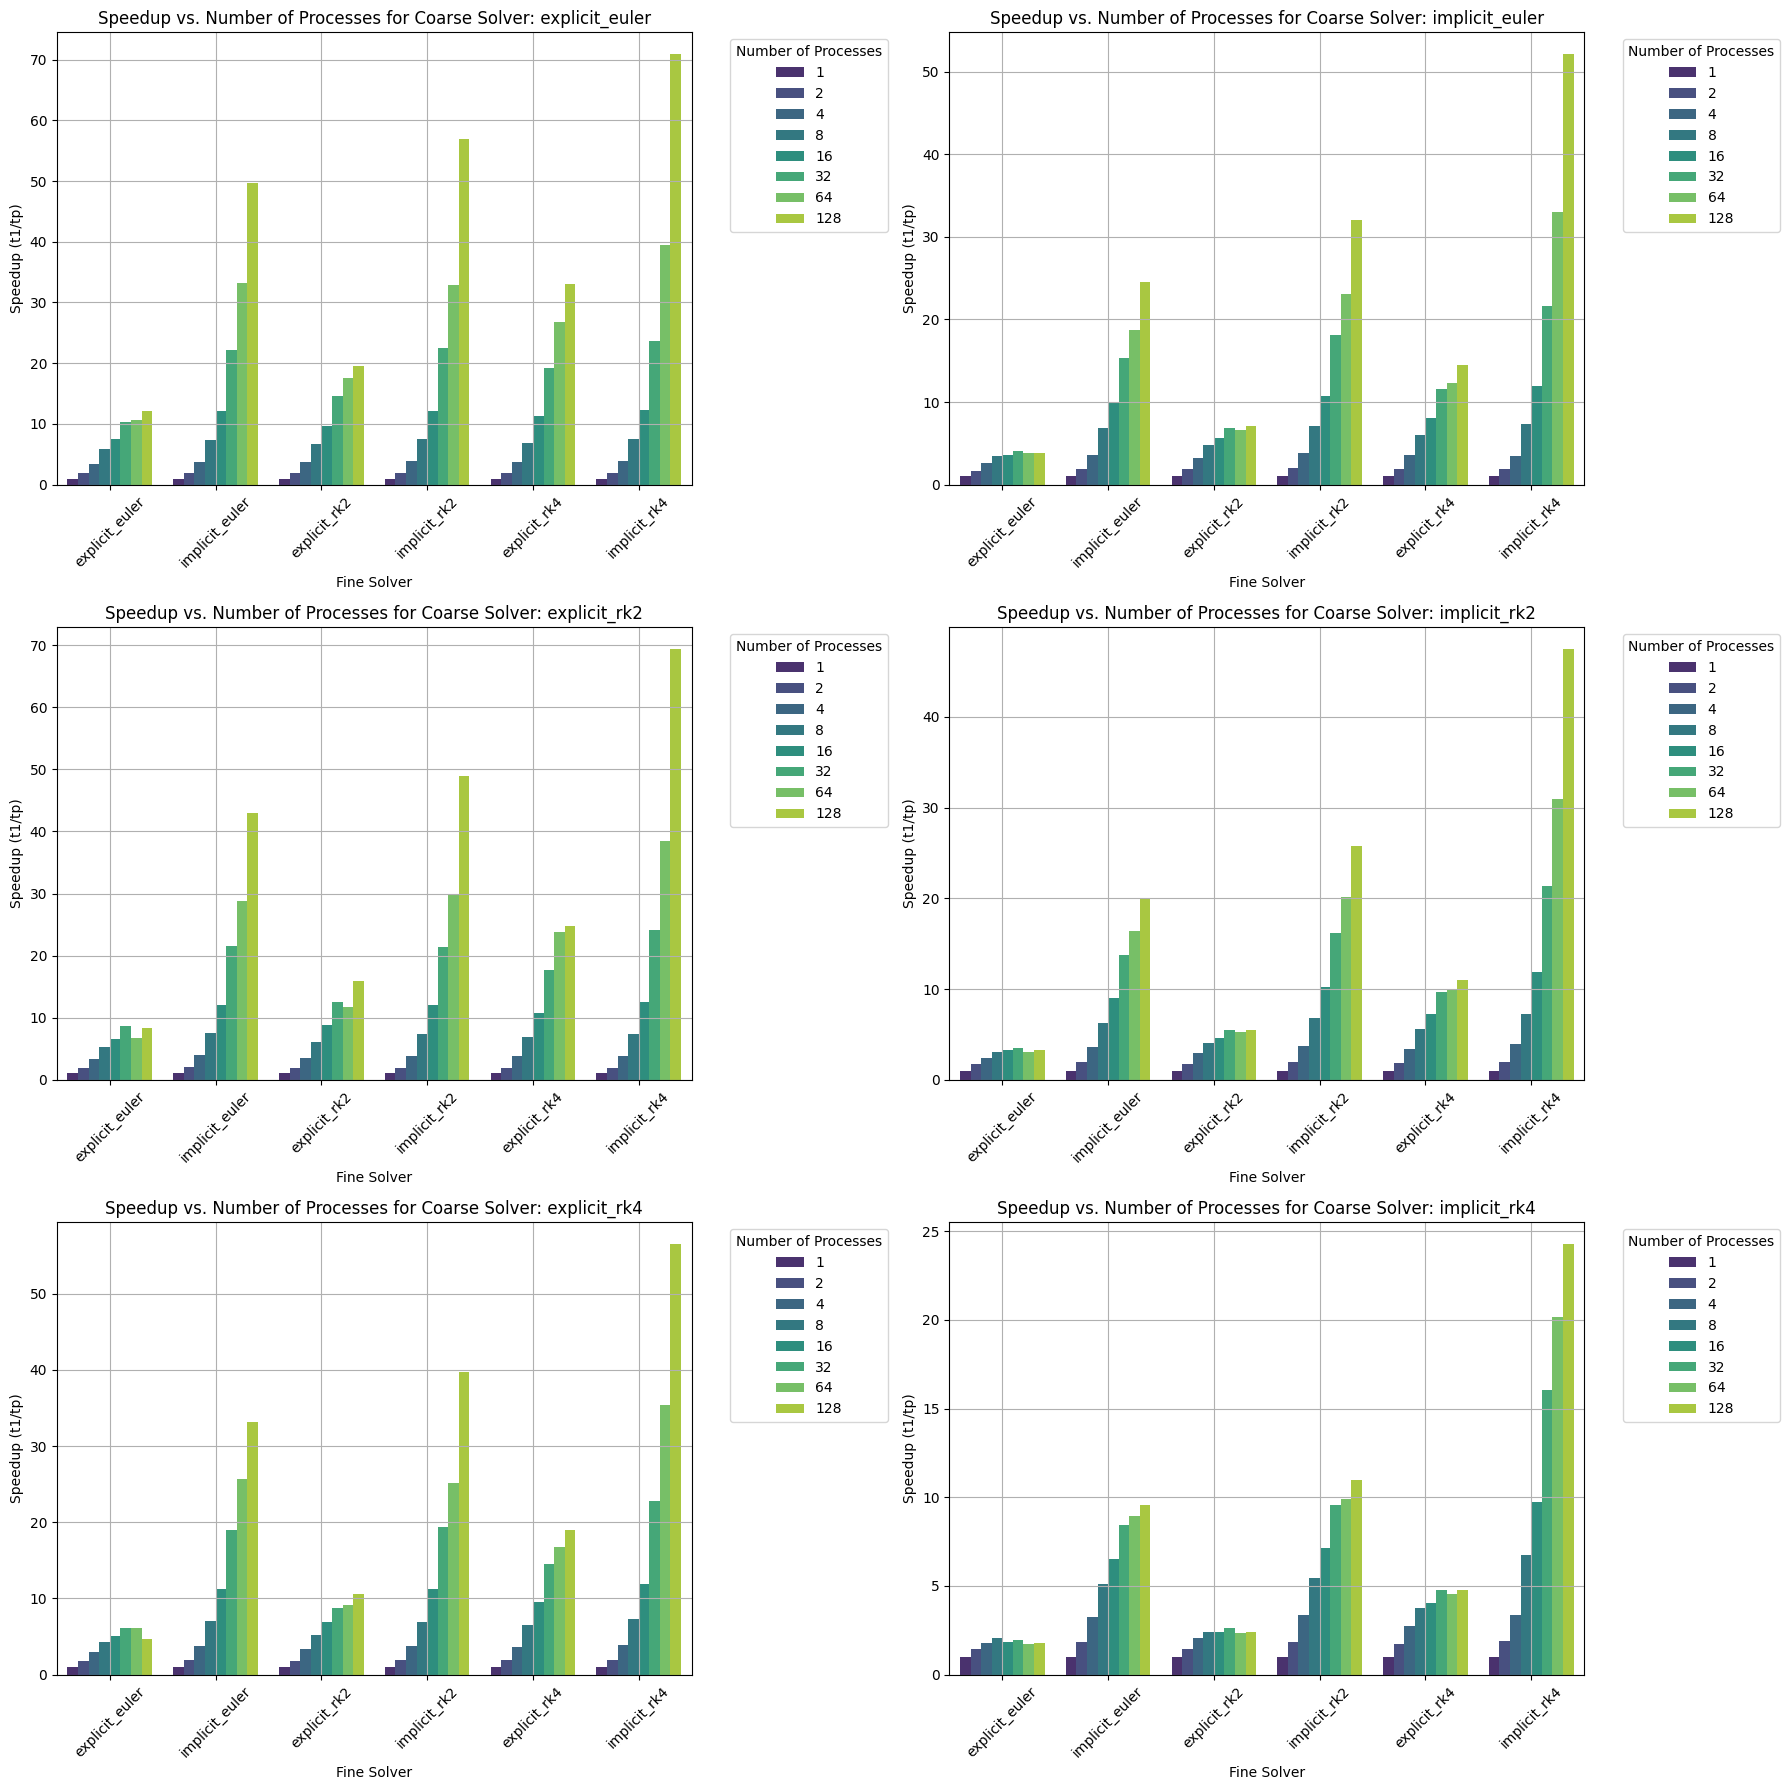
\includegraphics[width=1\textwidth]{img/perf.png}
    \caption{Speedup vs. Number of Processes for Different solvers combination}
    \label{fig:7}
\end{figure}
\newpage
\textbf{Analysis:}
\begin{itemize}
    \item The execution time decreased significantly as the number of processes increased, demonstrating the efficiency of parallel execution.
    \item The speedup achieved was nearly linear for a smaller number of processes but exhibited diminishing returns as the number of processes increased, particularly for explicit solvers. This is likely due to communication overhead and the shorter execution time of these methods, which limits further speed increases.
\end{itemize}

\section{Discussion}
The results of this study offer valuable insights into the performance and efficiency of the Parareal algorithm when applied to various systems with different solver combinations. Key findings and their implications are discussed below:
\subsection{Convergence Analysis}
The convergence analysis revealed that the number of iterations required for the Parareal algorithm to reach the specified tolerance varies significantly based on the solver combination used. 

Higher-order coarse solvers were shown to generally require fewer iterations for convergence compared to lower-order solvers. This indicates that the choice of coarse solver is crucial for optimizing the convergence rate of the Parareal algorithm. The efficiency gains from using higher-order coarse solvers, however, must be balanced against their increased computational complexity.
\subsection{Order of Convergence}
The analysis of the order of convergence demonstrated that the fine solver predominantly determines the Parareal algorithm’s convergence order, as discussed in Gunnar A. Staff's article (2002) \cite{staff2003convergence}. 

Higher-order fine solvers, such as RK4, resulted in a higher overall convergence order for the algorithm. This underlines the importance of selecting an appropriate fine solver to maximize the accuracy and efficiency of the Parareal algorithm. The results affirm that while higher-order solvers improve convergence properties, they also introduce greater computational demands. Therefore, the trade-off between accuracy and computational cost needs careful consideration when choosing solvers for the Parareal algorithm.

\newpage
\subsection{Performance Evaluation}
Performance evaluation using the Lorenz system showed a significant decrease in execution time as the number of processes increased, indicating the efficiency of parallel execution.

The speedup achieved was nearly linear for a smaller number of processes but exhibited diminishing returns as the number of processes increased, particularly for explicit solvers. This is likely due to communication overhead and the shorter execution time of explicit methods, which limits further speed increases. These findings suggest that while the Parareal algorithm can achieve substantial computational savings through parallelization, the efficiency gains may be limited by communication costs as the number of processes increases. Optimizing the balance between computation and communication is essential for maximizing the performance of the Parareal algorithm in large-scale parallel environments.
% --------------------------------------------------------------
%                            Conclusion
% --------------------------------------------------------------
\newpage
\section{Conclusion}
This study, hosted by Cemosis, extended previous work on the Parareal algorithm by thoroughly investigating its convergence properties, order of convergence, and performance in a parallel computing environment. The following conclusions can be drawn from the research:

\begin{enumerate}
    \item \textbf{Convergence Analysis:} The number of iterations required for convergence is significantly influenced by the choice of coarse solver. Higher-order coarse solvers generally lead to faster convergence. However, this improvement must be weighed against the increased computational demands of these solvers.
    \item \textbf{Order of Convergence:} The fine solver dictates the overall convergence order of the Parareal algorithm. Higher-order fine solvers enhance accuracy and improve the convergence rate. This finding highlights the importance of selecting an appropriate fine solver to optimize the algorithm’s performance.
    \item \textbf{Performance Evaluation:} Parallel execution significantly reduces execution time, demonstrating near-linear speedup with a smaller number of processes. However, as the number of processes increases, the speedup shows diminishing returns, especially for explicit solvers, due to communication overhead and the shorter execution times of these methods. This underscores the need for balancing computation and communication to maximize the efficiency of the Parareal algorithm.
\end{enumerate}\\

These findings underscore the importance of selecting appropriate solvers to optimize the performance and accuracy of the Parareal algorithm. Future work could further explore the application of adaptive solver strategies and investigate the algorithm's performance on more complex, real-world problems. Additionally, addressing communication overhead in large-scale parallel environments remains a crucial area for further research.

Overall, this study contributes to a deeper understanding of how different solvers impact the Parareal algorithm's efficiency and effectiveness, providing a foundation for optimizing parallel-in-time computations in scientific and engineering applications.

\newpage
% --- Biblio par .bib
\bibliography{ref.bib}
\vspace*{\fill}
%\selectlanguage{french}

%\begin{thebibliography}{7}
%\bibitem[Bastien 2019]{id-de-la-source}
%Auteurs : \emph{Un titre},  une date.
%\end{thebibliography}


\end{document}
